% !TeX root = ../../../main.tex
\section{Results}

Figure~\ref{fig:example} shows representative examples of acquired images from all four cohorts of kidneys and of all imaging modalities. All images were taken with the transducer in the 0 degree orientation, with parametric images of VisR RE, RV, DoPIo times-intersect, and shear elasticity estimates shown overlaid on top of B-modes. Where there are appreciable differences, the VisR and DoPIo images show (visco)elastic differences in similar locations. For example, in the combined injury example (4th row), the medulla appears as a soft feature while the cortex appears to its right as a stiffer feature.

\begin{sidewaysfigure}[!p]
    \centering
    \includegraphics[width=0.95\textheight]{parts/iri/figs/examples.eps}
    \caption{Example of acquired images for (top to bottom rows) an uninjured kidney as well as injured kidneys from the acute, chronic, and combined injury cohorts. Columns denote, from left to right, B-modes with renal capsule and medulla outlined in yellow, ARFI depth-normalized peak displacement, VisR RE, RV, DoPIo times-intersect, and DoPIo-estimated shear elasticity given the times-intersect in (c). Boxes denote sample ROIs used for the outer cortex (oC), inner cortex (iC), outer medulla (oM), and inner medulla (iM).}
    \label{fig:example}
\end{sidewaysfigure}

The distribution of VisR RE, RV, and DoPIo modulus parameters seen in Figure \ref{fig:example}, as well as those from all other acquisitions, are depicted as box plots in Figures \ref{fig:boxplotRe}, \ref{fig:boxplotRv}, and \ref{fig:boxplotDopio}, respectively. Note that each box for injured kidneys represents data pooled from three repeated acquisitions of images for five pigs in each injury cohort (i.e. 15 total acquisitions per box) whereas boxes for uninjured kidneys represent data pooled from three repeated acquisitions of images for both kidneys of three uninjured pigs (i.e. 18 total acquisitions per box).

\begin{figure}[!p]
    \centering
    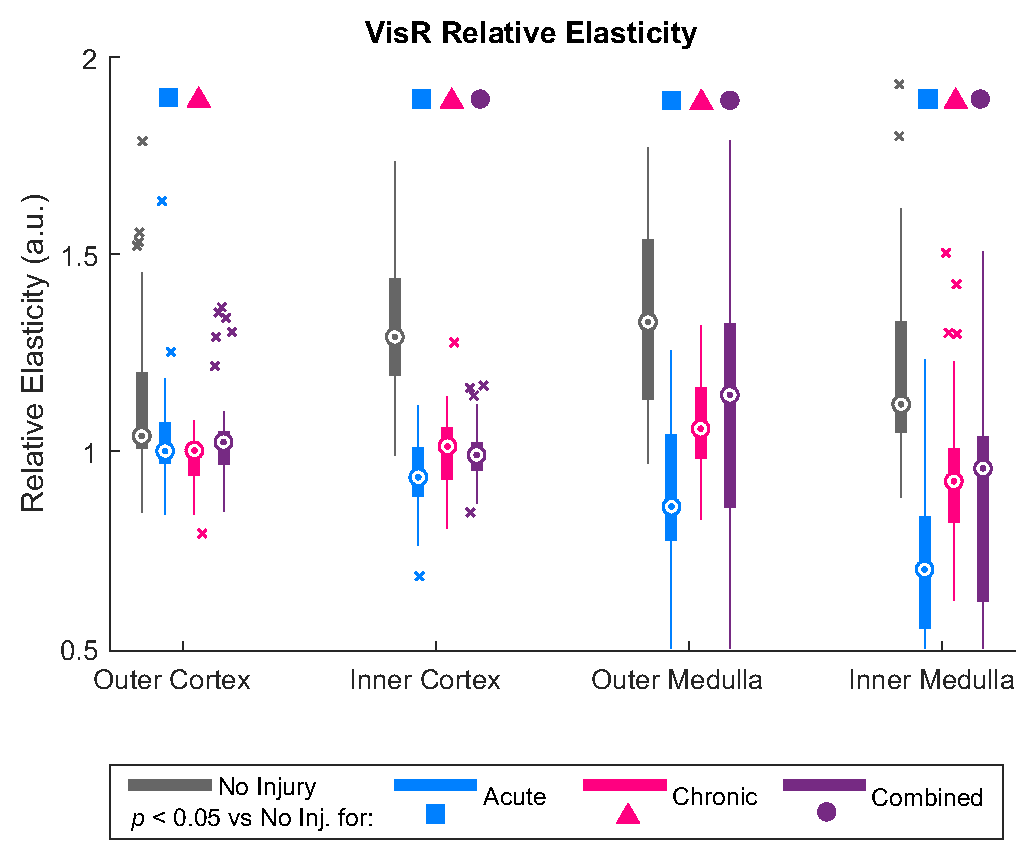
\includegraphics[width=0.8\textwidth]{parts/iri/figs/re.eps}
    \caption{Box plots of VisR RE values collected in various regions of porcine renal parenchyma for kidneys of uninjured pigs and the injured pigs from each injury cohort. The boxes represent the interquartile range (IQR) of the data, with the median value indicated by the circle within the box. Whiskers represent the range of the data up to the 95\% confidence interval, with outliers indicated by the crosses. Results of the Kruskal-\allowbreak{}Wallis test and Bonferroni post-hoc analyses for each anatomical region versus control kidneys are indicated by the shapes above the boxes.}
    \label{fig:boxplotRe}
\end{figure}
\begin{figure}[!p]
    \centering
    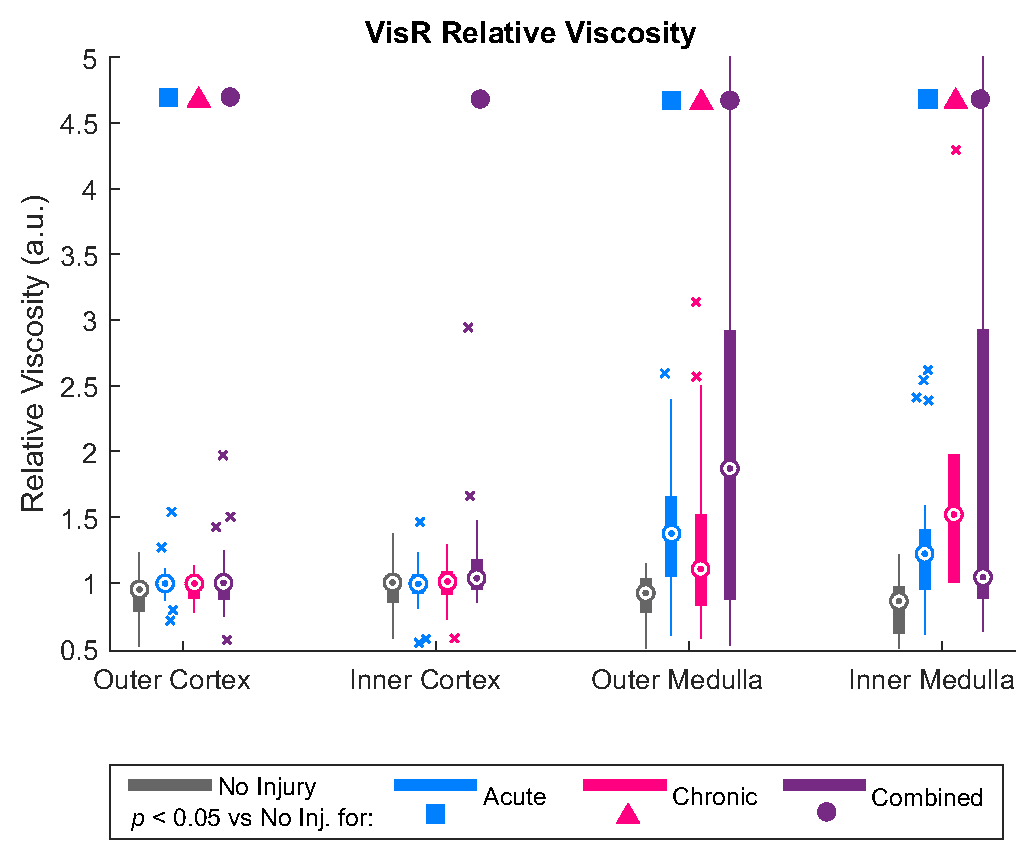
\includegraphics[width=0.8\textwidth]{parts/iri/figs/rv.eps}
    \caption{Box plots of VisR RV values collected in various regions of porcine renal parenchyma for kidneys of uninjured pigs and the injured pigs from each injury cohort. The boxes represent the interquartile range (IQR) of the data, with the median value indicated by the circle within the box. Whiskers represent the range of the data up to the 95\% confidence interval, with outliers indicated by the crosses. Results of the Kruskal-\allowbreak{}Wallis test and Bonferroni post-hoc analyses for each anatomical region versus control kidneys are indicated by the shapes above the boxes.}
    \label{fig:boxplotRv}
\end{figure}
\begin{figure}[!p]
    \centering
    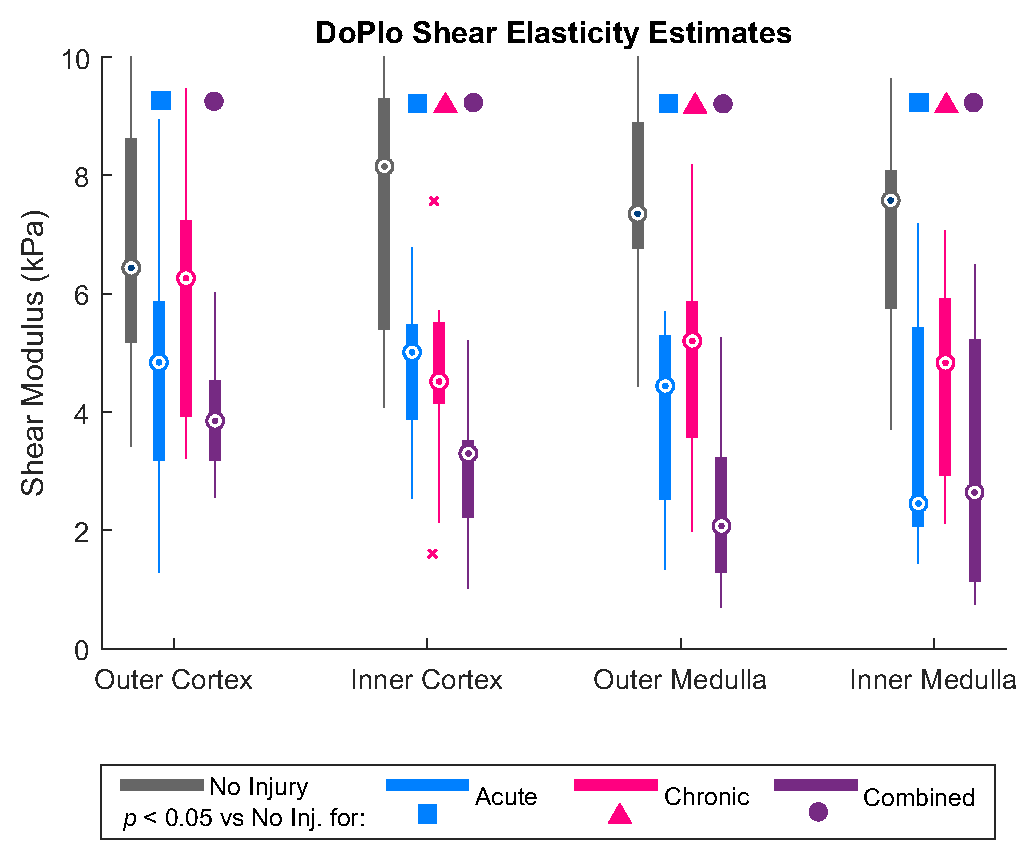
\includegraphics[width=0.8\textwidth]{parts/iri/figs/dopio.eps}
    \caption{Box plots of DoPIo shear elastic modulus estimates collected in various regions of porcine renal parenchyma for kidneys of uninjured pigs and the injured pigs from each injury cohort. The boxes represent the interquartile range (IQR) of the data, with the median value indicated by the circle within the box. Whiskers represent the range of the data up to the 95\% confidence interval, with outliers indicated by the crosses. Results of the Kruskal-Wallis test and Bonferroni post-hoc analyses for each anatomical region versus control kidneys are indicated by the shapes above the boxes.}
    \label{fig:boxplotDopio}
\end{figure}

Natural logarithms of DoA metrics (i.e. ln(DoA)) for VisR and DoPIo are shown in Figures \ref{fig:boxplotReDoa}, \ref{fig:boxplotRvDoa}, and \ref{fig:boxplotDopioDoa}. DoA measurements were taken as ratios between elasticity or viscosity measurements taken at 0 degree transducer orientations versus those from 90 degree orientations for each of three acquisitions (e.g. 0 / 90 degrees for the first, second, and third repeated acquisitions of each pig cohort). Note that in DoA measurements, the 0 degree orientation can appear stiffer than the 90 degree orientation in some cases, leading the ln(DoA) value to be negative. Note that this change in expression is unaffected for the Kruskal-Wallis test since the ranks of values in each distribution are unchanged.

\begin{figure}[!p]
    \centering
    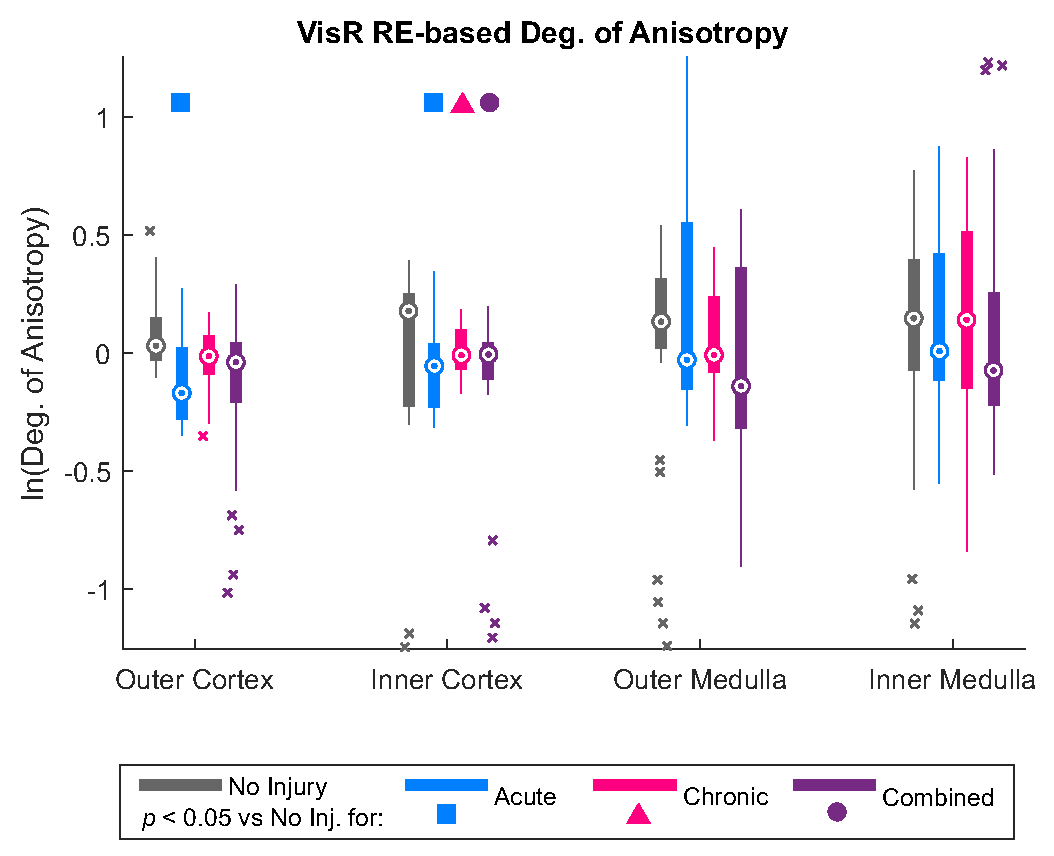
\includegraphics[width=0.8\textwidth]{parts/iri/figs/reDoA.eps}
    \caption{Box plots of ln(DoA) calculated from VisR RE values in various regions of porcine renal parenchyma. The boxes represent the interquartile range (IQR) of the data, with the median value indicated by the circle within the box. Whiskers represent the range of the data up to the 95\% confidence interval, with outliers indicated by the crosses. Results of the Kruskal-Wallis test and Bonferroni post-hoc analyses for each anatomical region versus control kidneys are indicated by the shapes above the boxes.}
    \label{fig:boxplotReDoa}
\end{figure}
\begin{figure}[htbp]
    \centering
    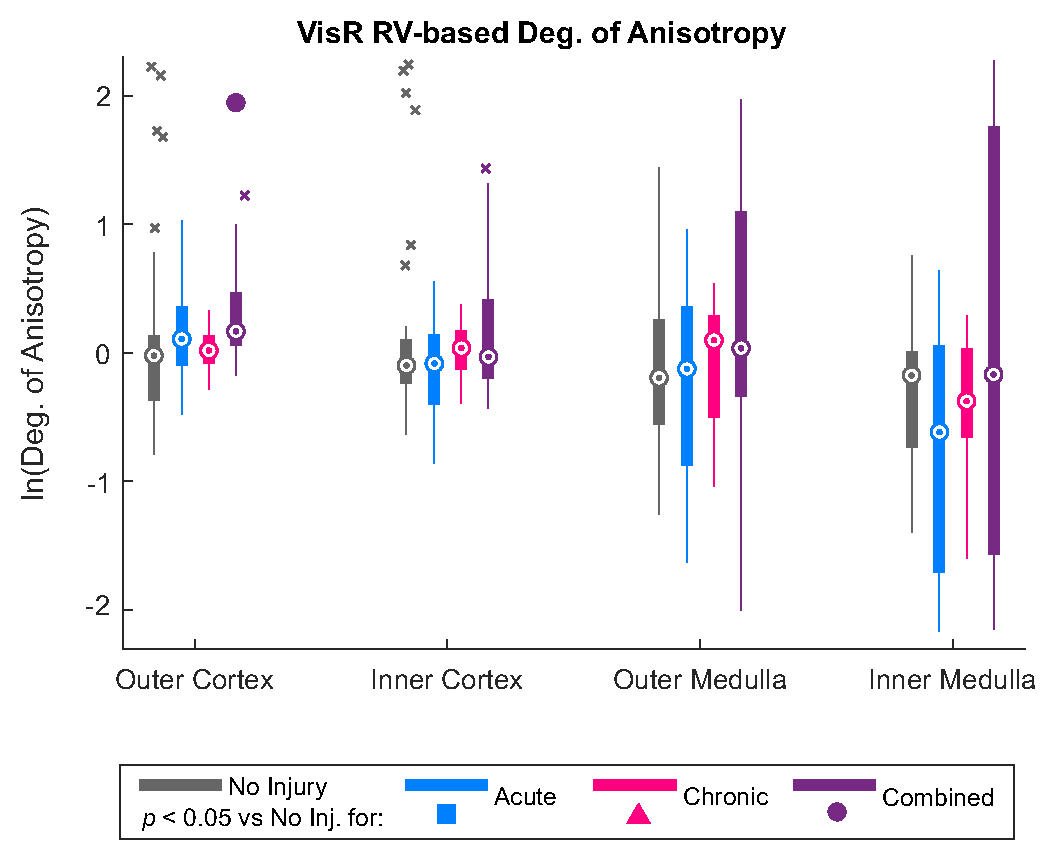
\includegraphics[width=0.8\textwidth]{parts/iri/figs/rvDoA.eps}
    \caption{Box plots of ln(DoA) calculated from VisR RV values in various regions of porcine renal parenchyma. The boxes represent the interquartile range (IQR) of the data, with the median value indicated by the circle within the box. Whiskers represent the range of the data up to the 95\% confidence interval, with outliers indicated by the crosses. Results of the Kruskal-Wallis test and Bonferroni post-hoc analyses for each anatomical region versus control kidneys are indicated by the shapes above the boxes.}
    \label{fig:boxplotRvDoa}
\end{figure}
\begin{figure}[!p]
    \centering
    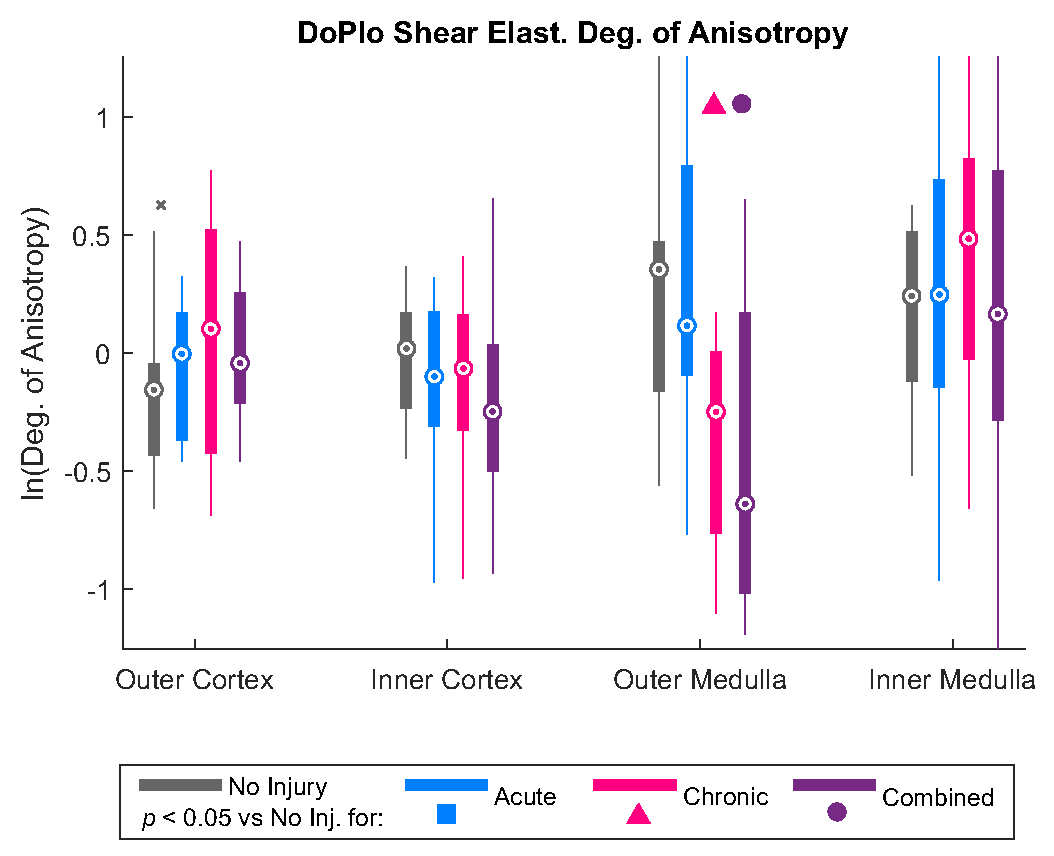
\includegraphics[width=0.8\textwidth]{parts/iri/figs/dopioDoA.eps}
    \caption{Box plots of ln(DoA) calculated from DoPIo shear elasticity estimates in various regions of porcine renal parenchyma. The boxes represent the interquartile range (IQR) of the data, with the median value indicated by the circle indicated within the box. Whiskers represent the range of the data up to the 95\% confidence interval, with outliers indicated by the crosses. Results of the Kruskal-Wallis test and Bonferroni post-hoc analyses for each anatomical region versus control kidney are indicated by the shapes above the boxes.}
    \label{fig:boxplotDopioDoa}
\end{figure}

Similarly, logarithmically transformed RR metrics, ln(RR), for VisR and DoPIo were calculated and plotted in Figures \ref{fig:boxplotReRr}, \ref{fig:boxplotRvRr}, and \ref{fig:boxplotDopioRr}. RR measurements were taken solely at the 0 degree transducer orientation, and calculated as ratios between elasticity measurements taken in one anatomical region versus another anatomical region in the same acquisition (e.g. outer cortex versus inner cortex for a given pig cohort and acquisition). If a VisR RE or RV values or DoPIo modulus estimate has a higher elasticity metric in the more superficial feature, it is plotted higher on the vertical axis; likewise, an RR value is plotted lower if a deeper feature has the dominant elasticity metric. The AUCs of classifiers using these inputs are shown in Fig~\ref{fig:auc}. Sensitivity and specificity are not shown, but specificity is considerably higher than sensitivity in most cases.

Representative examples of pathology slides from the cortex and medulla of the four cohorts are shown in Fig.~\ref{fig:histo}. Summary statistics of the ordinal scores are shown in Table~\ref{tbl:histoQuant}, with the median and median absolute deviation (MAD) of each finding listed for each cohort. Microscopic findings were consistent with expected injuries due to IRI. All microscopic findings were based on H\&E slides unless marked otherwise. Inflammation scores were based on the presence of mononuclear cell infiltrates in the cortical and medullary interstitia. No sex differences in findings were identified. Note that one contralateral kidney from the acute injury cohort was excluded from analysis due to the presence of unanticipated mild interstitial inflammation, tubular epithelial hyperplasia, and epithelial intranuclear inclusions as the result of a porcine adenovirus infection. Contralateral kidneys are listed in Table~\ref{tbl:histoQuant} solely to demonstrate their difference from truly-uninjured controls, and are not quantitatively compared elsewhere in this work.

\begin{figure}[!p]
    \centering
    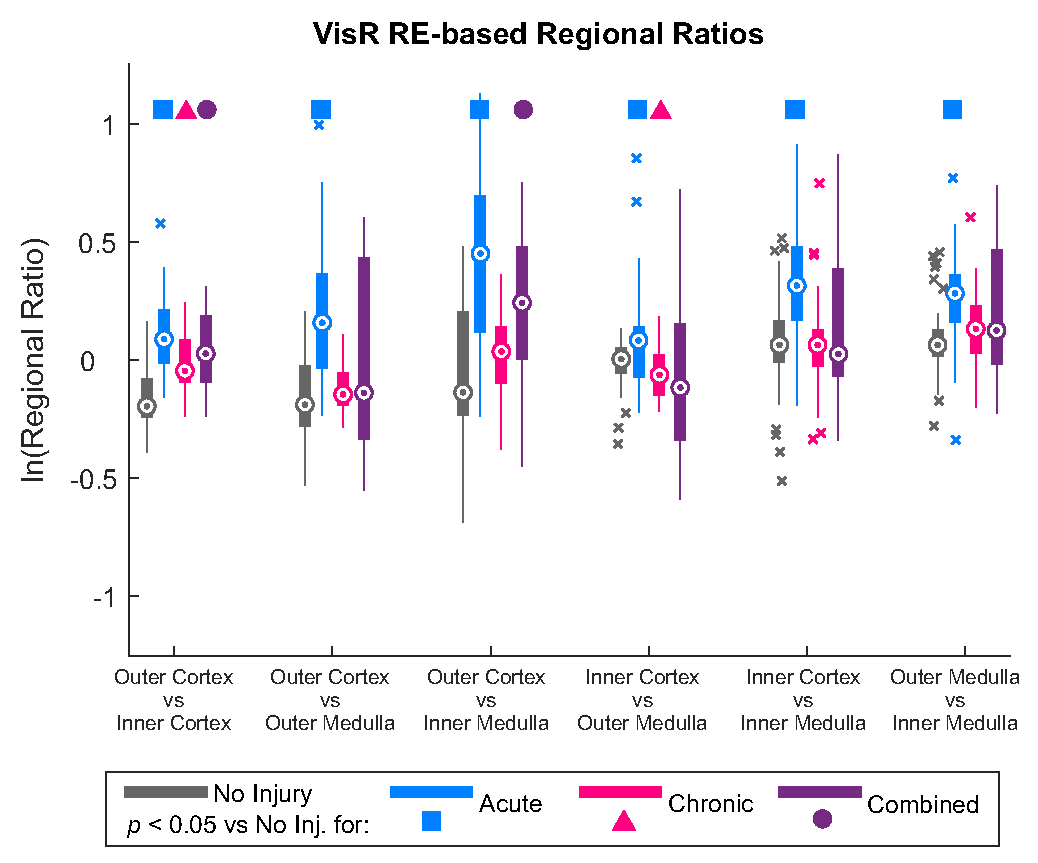
\includegraphics[width=0.8\textwidth]{parts/iri/figs/reRR.eps}
    \caption{Box plots of ln(RR) calculated from VisR relative elasticity values in various regions of porcine renal parenchyma. The boxes represent the interquartile range (IQR) of the data, with the median value indicated by the circle within the box. Whiskers represent the range of the data up to the 95\% confidence interval, with outliers indicated by the crosses. Results of the Kruskal-\allowbreak{}Wallis test and Bonferroni post-hoc analyses for each anatomical region versus control kidneys are indicated by the shapes above the boxes.}
    \label{fig:boxplotReRr}
\end{figure}
\begin{figure}[!p]
    \centering
    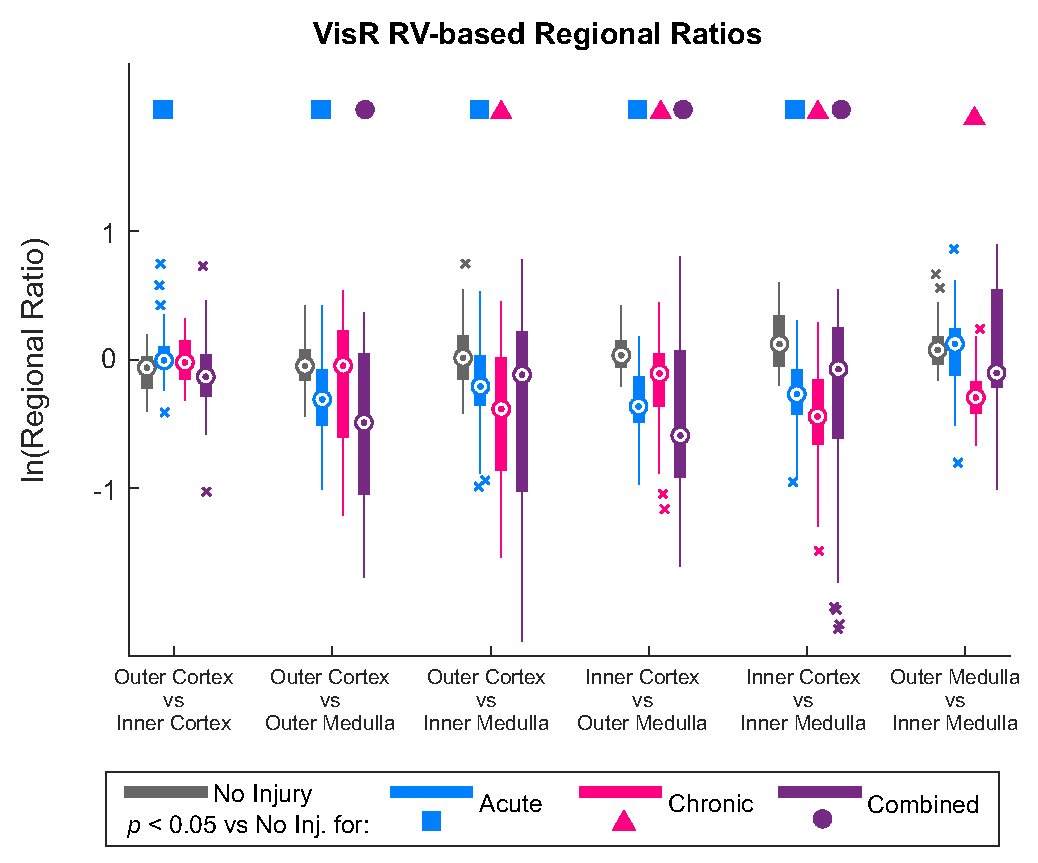
\includegraphics[width=0.8\textwidth]{parts/iri/figs/rvRR.eps}
    \caption{Box plots of ln(RR) calculated from VisR relative viscosity values in various regions of porcine renal parenchyma. The boxes represent the interquartile range (IQR) of the data, with the median value indicated by the circle within the box. Whiskers represent the range of the data up to the 95\% confidence interval, with outliers indicated by the crosses. Results of the Kruskal-\allowbreak{}Wallis test and Bonferroni post-hoc analyses for each anatomical region versus control kidneys are indicated by the shapes above the boxes.}
    \label{fig:boxplotRvRr}
\end{figure}
\begin{figure}[!p]
    \centering
    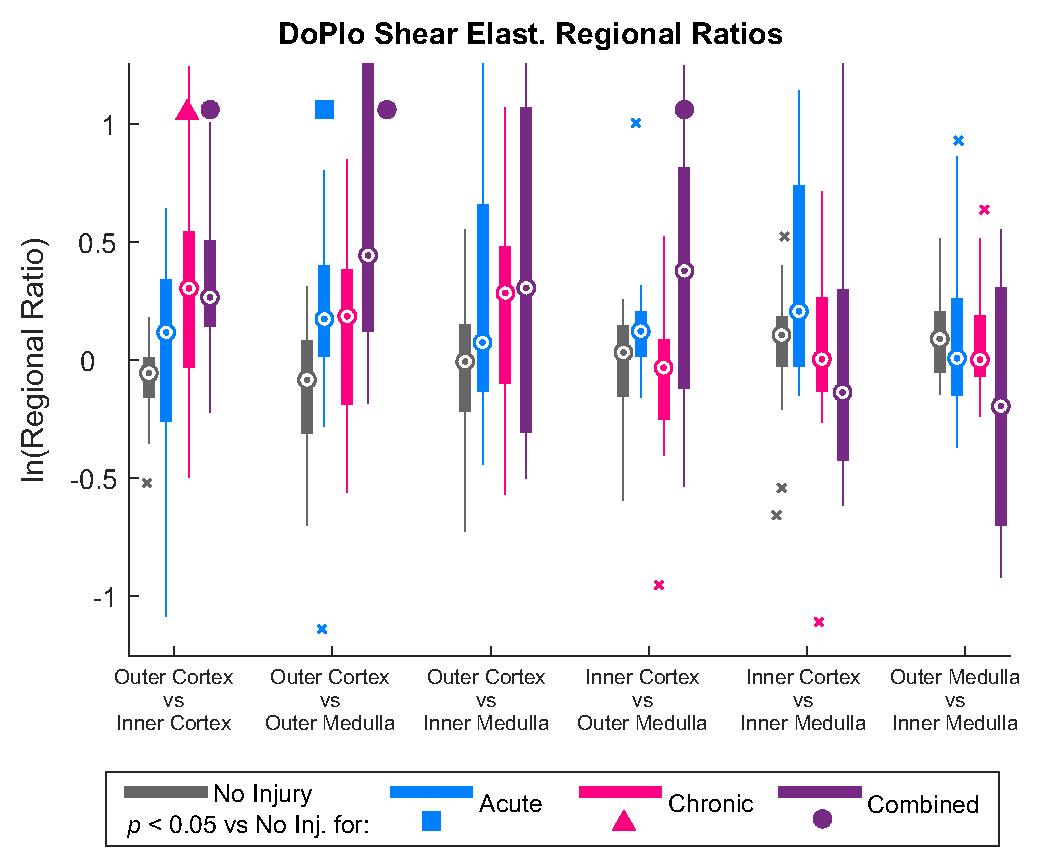
\includegraphics[width=0.8\textwidth]{parts/iri/figs/dopioRR.eps}
    \caption{Box plots of ln(RR) calculated from DoPIo shear elasticity estimates in various regions of porcine renal parenchyma. The boxes represent the interquartile range (IQR) of the data, with the median value indicated by the circle within the box. Whiskers represent the range of the data up to the 95\% confidence interval, with outliers indicated by the crosses. Results of the Kruskal-Wallis test and Bonferroni post-hoc analyses for each anatomical region versus control kidneys are indicated by the shapes above the boxes.}
    \label{fig:boxplotDopioRr}
\end{figure}

\begin{figure}[!p]
    \centering
    \includegraphics[width=\textwidth]{parts/iri/figs/histo.eps}
    \caption{Representative examples of histology slides of the renal cortex. From top to bottom, each row shows the inner medulla of kidneys from (1) the uninjured control cohort, as well as injured kidneys from the (2) acute injury, (3) chronic injury, and (4) combined injury cohorts. For each row, columns of images show sections with stains for (1) H\&E to show general tissue morphology, (2) picro-Sirius red to highlight areas with collagen, and (3) anti-Iba1 stains to indicate macrophage infiltration. Black bars on the bottom right of each image indicate scales of 50 \textmu{}m.}
    \label{fig:histo}
\end{figure}

%% !TeX root = ../../../main.tex

\begin{landscape}
    \singlespacing
    \centering
    \fontsize{8.5}{10}\selectfont
    \begin{longtable}{
        p{0.50in} 
        p{0.80in} | 
        p{0.70in} p{0.75in} | 
        p{0.70in} p{0.75in} | 
        p{0.70in} p{0.75in} | 
        p{0.70in} p{0.75in}}
        \caption{Performance of binary classification of renal IRI types using VisR versus DoPIo-derived metrics}\\
        \label{tbl:auc}\\
        \toprule
        \textbf{} &
        \textbf{} &
        \multicolumn{2}{c|}{\textbf{Any Injuries}} &
        \multicolumn{2}{c|}{\textbf{Acute Injuries}} &
        \multicolumn{2}{c|}{\textbf{Chronic Injuries}} &
        \multicolumn{2}{c}{\textbf{Combined Injuries}} \\
        \textbf{Modality} &
        \textbf{Analysis} &
        \textbf{AUC} &
        \textbf{ROIs Used} &
        \textbf{AUC} &
        \textbf{ROIs Used} &
        \textbf{AUC} &
        \textbf{ROIs Used} &
        \textbf{AUC} &
        \textbf{ROIs Used} \\ 
        \midrule
        \endfirsthead
        \endhead
        \endlastfoot
        VisR &
        RE only &
        0.62 ± 0.10 &
        oC &
        0.69 ± 0.14 &
        oM &
        \textbf{*0.69 ± 0.13} &
        \textbf{oC} &
        0.54 ± 0.17 &
        oM \\
        DoPIo &
        Modulus (G) only &
        \textbf{*0.83 ± 0.05} &
        \textbf{iM} &
        0.68 ± 0.04 &
        iM &
        0.56 ± 0.06 &
        oM &
        \textbf{*0.85 ± 0.03} &
        \textbf{oM} \\ \hline
        VisR &
        RR only &
        0.61 ± 0.09 &
        oC iC oM iM &
        0.71 ± 0.06 &
        oC iC iM &
        0.65 ± 0.11 &
        iC oM &
        0.67 ± 0.16 &
        iC oM \\
        DoPIo &
        RR only &
        \textbf{*0.66 ± 0.05} &
        \textbf{oC oM} &
        0.70 ± 0.07 &
        iC iM &
        0.57 ± 0.07 &
        oM iM &
        0.65 ± 0.08 &
        oM iM \\ \hline
        VisR &
        DoA only &
        0.64 ± 0.07 &
        iM &
        0.46 ± 0.10 &
        oC oM &
        0.56 ± 0.14 &
        iM &
        0.52 ± 0.16 &
        iM \\
        DoPIo &
        DoA only &
        0.67 ± 0.06 &
        oM &
        \textbf{*0.59 ± 0.09} &
        \textbf{oM} &
        0.60 ± 0.08 &
        oM &
        0.65 ± 0.06 &
        iC \\ \hline
        VisR &
        RE + RR &
        0.58 ± 0.12 &
        oC iC oM iM &
        0.73 ± 0.13 &
        iC oM iM &
        \textbf{*0.69 ± 0.13} &
        \textbf{oC iC iM} &
        0.59 ± 0.22 &
        iC oM iM \\
        DoPIo &
        G + RR &
        \textbf{*0.80 ± 0.08} &
        \textbf{oC iC iM} &
        0.55 ± 0.11 &
        iC oM iM &
        0.59 ± 0.08 &
        oC iC oM &
        \textbf{*0.83 ± 0.03} &
        \textbf{oC iC oM} \\ \hline
        VisR &
        RE + DoA &
        0.63 ± 0.13 &
        oC iC iM &
        0.73 ± 0.13 &
        iC oM &
        \textbf{*0.69 ± 0.13} &
        \textbf{oC iC} &
        0.59 ± 0.22 &
        oM iM \\
        DoPIo &
        G + DoA &
        \textbf{*0.80 ± 0.08} &
        \textbf{oC iC iM} &
        0.55 ± 0.11 &
        iC oM iM &
        0.59 ± 0.08 &
        oC oM &
        0.76 ± 0.05 &
        oC oM iM \\ \hline
        VisR &
        RR + DoA &
        0.51 ± 0.13 &
        iC oM iM &
        0.69 ± 0.17 &
        oC iC oM iM &
        0.59 ± 0.12 &
        oC oM iM &
        0.55 ± 0.23 &
        oC iC oM iM \\
        DoPIo &
        RR + DoA &
        0.61 ± 0.07 &
        oC iC oM iM &
        0.66 ± 0.07 &
        oC iC oM iM &
        0.58 ± 0.08 &
        oC iC oM iM &
        0.63 ± 0.09 &
        oC iC oM iM \\ \hline
        VisR &
        RE + RR + DoA &
        0.62 ± 0.14 &
        oC iC iM &
        0.70 ± 0.13 &
        oC iC oM iM &
        0.69 ± 0.13 &
        oC iC iM &
        0.57 ± 0.22 &
        iC oM iM \\
        DoPIo &
        G + RR + DoA &
        \textbf{*0.82 ± 0.05} &
        \textbf{iC oM iM} &
        0.64 ± 0.06 &
        iC oM iM &
        0.56 ± 0.08 &
        oC iC oM iM &
        \textbf{*0.80 ± 0.08} &
        \textbf{oC iC oM iM} \\ 
        \bottomrule
    \end{longtable}
    \par\vspace{0.5em}
    \noindent{}AUC is reported as median ± median absolute deviation (MAD); asterisks denote the higher median where AUC distributions were significantly different between the best VisR- versus DoPIo-based classifiers. Inputs that gave the best performance for each injury type and input type are indicated below the performance metrics, with "i" indicating an "inner" part of a renal structure, "o" for outer, "C" for cortex, and "M" for medulla.
\end{landscape}

\begin{figure}[!p]
    \centering
    \includegraphics[width=0.8\textwidth]{parts/iri/figs/auc.eps}
    \caption{Bar graph of AUC for binary classifiers of (a) measurements from kidneys with any injury, as well as measurements specifically from the (b) acute, (c) chronic, and (d) combined injury cohorts, using the best combination of VisR RE, RV, or DoPIo-derived metrics as inputs. AUC is reported as median ± median absolute deviation (MAD). Gray bars indicate pairs of AUC distributions that were found to be significantly different from a Kruskal-Wallis test and Bonferroni post-hoc analyses. Inputs that gave the best performance for each injury type and input type are indicated next to the readout of plotted median AUC values, with "i" indicating an "inner" part of a renal structure, "o" for outer, "C" for cortex, and "M" for medulla.}
    \label{fig:auc}
\end{figure}

\afterpage{%
    \clearpage
    % !TeX root = ../../../main.tex

\begin{landscape}
    \singlespacing
    \fontsize{8.5}{9}\selectfont
    \centering
    \begin{longtable}{p{0.50in}p{1.70in}|lcl|lcl|lcl|c}
        \caption{Pathologist scoring of observed pathologies in porcine renal parenchyma}
        \label{tbl:histoQuant}\\
        \toprule\\
        &  & \multicolumn{3}{c|}{\textbf{Acute Injury Cohort}} & \multicolumn{3}{c|}{\textbf{Chronic Injury Cohort}} & \multicolumn{3}{c|}{\textbf{Combined Injury Cohort}} & \multirow{2}{*}{\textbf{Uninjured Controls}} \\
        \multicolumn{1}{c}{} & \multicolumn{1}{c|}{} & Injured &  & Contralateral & Injured &  & Contralateral & Injured &  & Contralateral &  \\
        \textbf{Category} & \textbf{Microscopic Finding} & n = 10 &  & n = 9 & n = 10 &  & n = 10 & n = 10 &  & n = 10 & n = 12 \\ 
        \midrule
        \endfirsthead
        \endhead
        \endlastfoot
        Cortex & Inflammatory cell infiltrates, acute & \textbf{*1.0 ± 0.0} & † & 0.0 ± 0.0 & 0.0 ± 0.0 &  & 0.0 ± 0.0 & \textbf{*1.0 ± 0.0} & † & 0.0 ± 0.0 & 0.0 ± 0.0 \\
        & Interstitial edema & \textbf{*1.0 ± 0.2} & † & 0.0 ± 0.0 & 0.0 ± 0.0 &  & 0.0 ± 0.0 & \textbf{*2.0 ± 0.0} & † & 0.0 ± 0.0 & 0.0 ± 0.0 \\
        & Necrosis, tubular epithelium, acute & \textbf{*4.0 ± 0.0} & † & 0.0 ± 0.0 & 0.0 ± 0.0 &  & 0.0 ± 0.0 & \textbf{*4.0 ± 0.0} & † & 0.0 ± 0.0 & 0.0 ± 0.0 \\
        & Tubular degeneration/regeneration & \textbf{*4.0 ± 0.0} & † & 0.0 ± 0.0 & 0.0 ± 0.4 &  & 0.0 ± 0.2 & \textbf{*3.0 ± 0.0} & † & 0.0 ± 0.0 & 0.0 ± 0.0 \\
        & Neutrophilic infiltrates, intratubular & \textbf{*1.0 ± 0.2} & † & 0.0 ± 0.0 & 0.0 ± 0.0 &  & 0.0 ± 0.0 & \textbf{*1.0 ± 1.0} & † & 0.0 ± 0.0 & 0.0 ± 0.0 \\
        & Glomerulosclerosis, multifocal & 0 present &  & 0 present & \textbf{*8 present} & † & 0 present & \textbf{*7 present} & † & 0 present & 0 present \\
        & Macrophage distribution (Iba1) & \textbf{*4.0 ± 0.4} & † & \textbf{*2.0 ± 0.5} & \textbf{*2.0 ± 0.5} & † & \textbf{*1.0 ± 0.2} & \textbf{*4.0 ± 0.5} & † & \textbf{*1.0 ± 0.2} & 0.0 ± 0.0 \\
        & Fibrosis (picro-Sirius red) & \textbf{*1.0 ± 0.0} &  & \textbf{*2.0 ± 0.0} & \textbf{*2.5 ± 0.5} & † & \textbf{*1.0 ± 0.0} & \textbf{*3.0 ± 1.0} & † & 1.0 ± 0.0 & 0.0 ± 0.0 \\
        & Tubular drop-out & 0.0 ± 0.0 &  & 0.0 ± 0.0 & 0.0 ± 0.0 &  & 0.0 ± 0.0 & \textbf{*2.0 ± 1.0} & † & 0.0 ± 0.0 & 0.0 ± 0.0 \\ \hline
        Medulla & Inflammatory cell infiltrates, acute & \textbf{*1.0 ± 0.0} & † & 0.0 ± 0.0 & 0.0 ± 0.0 &  & 0.0 ± 0.0 & 0.0 ± 0.0 &  & 0.0 ± 0.0 & 0.0 ± 0.0 \\
        & Interstitial edema & \textbf{*1.0 ± 0.0} & † & 0.0 ± 0.0 & 0.0 ± 0.0 &  & 0.0 ± 0.0 & \textbf{*1.5 ± 0.5} &  & \textbf{*1.0 ± 1.0} & 0.0 ± 0.0 \\
        & Necrosis, tubular epithelium, acute & 0.0 ± 0.0 &  & 0.0 ± 0.0 & 0.0 ± 0.0 &  & 0.0 ± 0.0 & 0.0 ± 0.0 &  & 0.0 ± 0.0 & 0.0 ± 0.0 \\
        & Tubular degeneration/regeneration & \textbf{*0.0 ± 0.0} & † & 0.0 ± 0.0 & 0.0 ± 0.0 &  & 0.0 ± 0.0 & \textbf{*0.0 ± 0.7} & † & 0.0 ± 0.0 & 0.0 ± 0.0 \\
        & Tubular hyperplasia, multifocal & 0.0 ± 0.0 &  & 0.0 ± 0.0 & 0.0 ± 0.0 &  & 0.0 ± 0.0 & 0.0 ± 0.0 &  & 0.0 ± 0.0 & 0.0 ± 0.0 \\
        & Neutrophilic infiltrates, intratubular & \textbf{*1.0 ± 0.0} & † & 0.0 ± 0.0 & 0.0 ± 0.0 &  & 0.0 ± 0.0 & \textbf{*1.0 ± 0.0} & † & 0.0 ± 0.0 & 0.0 ± 0.0 \\
        & Macrophage distribution (Iba1) & \textbf{*3.5 ± 0.5} &  & \textbf{*3.0 ± 1.0} & \textbf{*1.5 ± 0.5} &  & \textbf{*1.0 ± 0.0} & \textbf{*3.5 ± 0.7} & † & 1.5 ± 0.6 & 0.0 ± 0.0 \\
        & Fibrosis (picro-Sirius red) & \textbf{*1.0 ± 0.0} &  & \textbf{*1.0 ± 0.0} & \textbf{*1.0 ± 0.6} &  & 0.5 ± 0.7 & 1.5 ± 0.9 &  & 1.0 ± 0.5 & 0.0 ± 0.0 \\ 
        \bottomrule
    \end{longtable}
    \par\vspace{0.5em}
    \noindent{}Values are reported as median ± median absolute deviation (MAD) for ordinal scores, or as counts for presence/absence findings. "n" refers to the number of histology slides per category. Bolded values with asterisks (*) are those that are significantly different from uninjured control kidneys. Daggers (\textdagger) indicate significant differences between injured and contralateral kidneys within the same injury cohort.
\end{landscape}

    \clearpage
}
